\documentclass[conference]{IEEEtran}
\IEEEoverridecommandlockouts
\usepackage{cite}
\usepackage{amsmath,amssymb,amsfonts}
\usepackage{algorithm}
\usepackage{algpseudocode}
\usepackage{graphicx}
\usepackage{booktabs}
\usepackage{array}
\usepackage{multirow}
\usepackage{xcolor}
\usepackage{tikz}
\usetikzlibrary{arrows.meta,positioning,fit}
\usepackage{url}
\newtheorem{proposition}{Proposition}
% Auto-generated by code/make_outputs.py from results/*.json -- do not edit.
\newcommand{\AlphaHiSy}{none}
\newcommand{\AlphaHiTr}{1.4}
\newcommand{\AlphaLoSy}{0.88}
\newcommand{\AlphaLoTr}{0.85}
\newcommand{\AlphaMax}{8}
\newcommand{\AlphaMin}{0.10}
\newcommand{\BoundWhole}{11}
\newcommand{\BoundWin}{21}
\newcommand{\BudHighAlpha}{0.44}
\newcommand{\BudHighRate}{6}
\newcommand{\BudN}{8}
\newcommand{\BudSyCiMax}{11}
\newcommand{\BudSyFgBeatsSchedB}{0}
\newcommand{\BudSyFgBeatsSchedC}{3}
\newcommand{\BudSyFgLow}{12.5}
\newcommand{\BudSyFgLowRate}{1.00}
\newcommand{\BudSyRrLow}{14.2}
\newcommand{\BudSyWinMin}{0.50}
\newcommand{\BudTrFgBeatsSchedB}{0}
\newcommand{\BudTrFgBeatsSchedC}{4}
\newcommand{\BudTrFgLow}{41.0}
\newcommand{\BudTrFgLowRate}{1.04}
\newcommand{\BudTrFgRateLowMax}{1.04}
\newcommand{\BudTrFgSensorLowMax}{1.13}
\newcommand{\BudTrRrLow}{38.3}
\newcommand{\BudTrSchedBBeatsFg}{8}
\newcommand{\BudTrSchedCBeatsFg}{4}
\newcommand{\BudTrWinMin}{1.00}
\newcommand{\CalFgObs}{0.27}
\newcommand{\CalFgPred}{0.27}
\newcommand{\CalGaussObs}{0.22}
\newcommand{\CalGaussPred}{0.39}
\newcommand{\EceFg}{0.05}
\newcommand{\EceGauss}{0.19}
\newcommand{\EpsHoH}{20}
\newcommand{\EpsHoOne}{38}
\newcommand{\EpsHoQ}{-15}
\newcommand{\EpsSyH}{28}
\newcommand{\EpsSyOne}{28}
\newcommand{\EpsSyQ}{16}
\newcommand{\EpsTrH}{15}
\newcommand{\EpsTrOne}{39}
\newcommand{\EpsTrQ}{-16}
\newcommand{\EpsVHoHFG}{7.7}
\newcommand{\EpsVHoHRR}{9.6}
\newcommand{\EpsVHoOneFG}{2.5}
\newcommand{\EpsVHoOneRR}{4.1}
\newcommand{\EpsVHoQFG}{23.3}
\newcommand{\EpsVHoQRR}{20.2}
\newcommand{\EpsVSyHFG}{2.9}
\newcommand{\EpsVSyHRR}{4.0}
\newcommand{\EpsVSyOneFG}{0.4}
\newcommand{\EpsVSyOneRR}{0.6}
\newcommand{\EpsVSyQFG}{11.4}
\newcommand{\EpsVSyQRR}{13.5}
\newcommand{\EpsVTrHFG}{9.9}
\newcommand{\EpsVTrHRR}{11.7}
\newcommand{\EpsVTrOneFG}{3.2}
\newcommand{\EpsVTrOneRR}{5.3}
\newcommand{\EpsVTrQFG}{25.8}
\newcommand{\EpsVTrQRR}{22.3}
\newcommand{\GainMorning}{79}
\newcommand{\GainMorningGross}{68}
\newcommand{\HeadCapSyFive}{5.10}
\newcommand{\HeadCapSyOne}{1.20}
\newcommand{\HeadCapSyOneHalf}{1.50}
\newcommand{\HeadCapSyThree}{3.00}
\newcommand{\HeadCapSyTwo}{2.10}
\newcommand{\HeadCapTrFive}{5.36}
\newcommand{\HeadCapTrOne}{1.07}
\newcommand{\HeadCapTrOneHalf}{2.14}
\newcommand{\HeadCapTrThree}{3.21}
\newcommand{\HeadCapTrTwo}{2.14}
\newcommand{\HeadKSyFive}{17}
\newcommand{\HeadKSyOne}{4}
\newcommand{\HeadKSyOneHalf}{5}
\newcommand{\HeadKSyThree}{10}
\newcommand{\HeadKSyTwo}{7}
\newcommand{\HeadKTrFive}{5}
\newcommand{\HeadKTrOne}{1}
\newcommand{\HeadKTrOneHalf}{2}
\newcommand{\HeadKTrThree}{3}
\newcommand{\HeadKTrTwo}{2}
\newcommand{\HeadSyFive}{27.9}
\newcommand{\HeadSyMax}{28}
\newcommand{\HeadSyMin}{23}
\newcommand{\HeadSyOne}{23.4}
\newcommand{\HeadSyOneHalf}{28.0}
\newcommand{\HeadSyThree}{27.6}
\newcommand{\HeadSyTwo}{27.8}
\newcommand{\HeadTrFive}{20.3}
\newcommand{\HeadTrMax}{20}
\newcommand{\HeadTrMin}{-4}
\newcommand{\HeadTrOne}{-4.5}
\newcommand{\HeadTrOneHalf}{17.5}
\newcommand{\HeadTrThree}{15.4}
\newcommand{\HeadTrTwo}{17.5}
\newcommand{\HoAoiFG}{20.8}
\newcommand{\HoAoiRR}{18.7}
\newcommand{\HoDPS}{7.52}
\newcommand{\HoDays}{7}
\newcommand{\HoDiff}{1.47}
\newcommand{\HoDiffCI}{[-1.00, 3.94]}
\newcommand{\HoDpsE}{0.92}
\newcommand{\HoDpsRed}{22}
\newcommand{\HoFG}{7.73}
\newcommand{\HoFailFG}{21}
\newcommand{\HoFailRR}{17}
\newcommand{\HoFgVsSchedB}{9}
\newcommand{\HoGauss}{8.01}
\newcommand{\HoHead}{3.75}
\newcommand{\HoK}{1}
\newcommand{\HoMV}{9.67}
\newcommand{\HoMotes}{8}
\newcommand{\HoMyo}{9.01}
\newcommand{\HoMyoRed}{7}
\newcommand{\HoNdays}{9}
\newcommand{\HoNoCap}{19.56}
\newcommand{\HoNoCapFail}{47}
\newcommand{\HoNoCapRate}{1.176}
\newcommand{\HoNoCapRed}{-103}
\newcommand{\HoNoProj}{7.94}
\newcommand{\HoOR}{2.38}
\newcommand{\HoObs}{84.1}
\newcommand{\HoRND}{20.86}
\newcommand{\HoRR}{9.65}
\newcommand{\HoRateMax}{1.002}
\newcommand{\HoRateMean}{0.988}
\newcommand{\HoRed}{20}
\newcommand{\HoSchedB}{7.12}
\newcommand{\HoSchedBExpo}{0.375}
\newcommand{\HoSchedBRed}{26}
\newcommand{\HoSchedBStat}{RR violation profile}
\newcommand{\HoSchedC}{8.72}
\newcommand{\HoSchedCExpo}{0.25}
\newcommand{\HoSchedCRed}{10}
\newcommand{\HoShape}{7.75}
\newcommand{\HoShared}{6}
\newcommand{\HoStart}{2004-03-12}
\newcommand{\HoStatic}{10.12}
\newcommand{\HoursWorse}{13}
\newcommand{\HoursWorseNight}{10}
\newcommand{\IntelClean}{1{,}784{,}239}
\newcommand{\IntelExpDay}{1.43}
\newcommand{\IntelExpNight}{1.29}
\newcommand{\IntelMotes}{28}
\newcommand{\IntelObs}{89.9}
\newcommand{\IntelParsed}{2{,}210{,}084}
\newcommand{\IntelRows}{2{,}313{,}682}
\newcommand{\IntelStart}{2004-02-29}
\newcommand{\LbFGtrend}{41.0}
\newcommand{\LbFGtrendRate}{1.04}
\newcommand{\LbFGzoh}{46.1}
\newcommand{\LbFGzohRate}{1.05}
\newcommand{\LbRRtrend}{38.3}
\newcommand{\LbRRtrendRate}{1.00}
\newcommand{\LbRRzoh}{45.0}
\newcommand{\LbRRzohRate}{1.00}
\newcommand{\LossTopHours}{12:00, 13:00, 16:00}
\newcommand{\LossTopShare}{56}
\newcommand{\LossWorstFG}{16.7}
\newcommand{\LossWorstHour}{12:00}
\newcommand{\LossWorstRR}{15.2}
\newcommand{\MyoLr}{0.02}
\newcommand{\MyoS}{10}
\newcommand{\MyoV}{200}
\newcommand{\NightFG}{31}
\newcommand{\NightRR}{46}
\newcommand{\NpVer}{2.5.3}
\newcommand{\OverMax}{18}
\newcommand{\OverMaxAbl}{18}
\newcommand{\PeakFG}{4.4}
\newcommand{\PeakHourFG}{07:00}
\newcommand{\PeakIsRRmax}{yes}
\newcommand{\PeakVFG}{32.7}
\newcommand{\PeakVRR}{45.7}
\newcommand{\PyVer}{3.13.17}
\newcommand{\QrunMax}{10.9}
\newcommand{\RRrate}{2}
\newcommand{\RegimeLoseAbove}{4}
\newcommand{\RegimeLoseAboveAll}{yes}
\newcommand{\RegimeLoseBelow}{3}
\newcommand{\RegimeThr}{24}
\newcommand{\RobHoMax}{27}
\newcommand{\RobHoMin}{13}
\newcommand{\RobTrMax}{31}
\newcommand{\RobTrMin}{4}
\newcommand{\RtFGbig}{381}
\newcommand{\RtFGmid}{132}
\newcommand{\RtFGsmall}{87}
\newcommand{\RtRRbig}{24}
\newcommand{\RtRRmid}{17}
\newcommand{\RtRRsmall}{22}
\newcommand{\SchHoCausal}{8.72}
\newcommand{\SchHoCausalExpo}{0.25}
\newcommand{\SchHoIncr}{8.04}
\newcommand{\SchHoIncrExpo}{0.375}
\newcommand{\SchHoRrv}{7.12}
\newcommand{\SchHoRrvExpo}{0.375}
\newcommand{\SchSyCausal}{2.79}
\newcommand{\SchSyCausalExpo}{0.75}
\newcommand{\SchSyIncr}{2.38}
\newcommand{\SchSyIncrExpo}{1}
\newcommand{\SchSyRrv}{2.42}
\newcommand{\SchSyRrvExpo}{1}
\newcommand{\SchTrCausal}{10.57}
\newcommand{\SchTrCausalExpo}{0.375}
\newcommand{\SchTrIncr}{10.88}
\newcommand{\SchTrIncrExpo}{0.25}
\newcommand{\SchTrRrv}{9.22}
\newcommand{\SchTrRrvExpo}{0.375}
\newcommand{\ShapeOn}{yes}
\newcommand{\SvHoPost}{7.27}
\newcommand{\SvHoPre}{7.73}
\newcommand{\SvTrPost}{8.04}
\newcommand{\SvTrPre}{9.88}
\newcommand{\SvValPost}{3.30}
\newcommand{\SvValPre}{3.07}
\newcommand{\SyAoiFG}{20.4}
\newcommand{\SyAoiRR}{14.5}
\newcommand{\SyDPS}{3.19}
\newcommand{\SyDpsE}{0.92}
\newcommand{\SyDpsEmin}{0.72}
\newcommand{\SyDpsHighAlpha}{15.44}
\newcommand{\SyDpsLowAlpha}{0.32}
\newcommand{\SyDpsRed}{23}
\newcommand{\SyDpsRedCI}{[22.6, 24.2]}
\newcommand{\SyFG}{3.03}
\newcommand{\SyFgHighAlpha}{14.16}
\newcommand{\SyFgLowAlpha}{1.48}
\newcommand{\SyFgVsSchedB}{24}
\newcommand{\SyGauss}{3.03}
\newcommand{\SyGaussDiff}{0.00}
\newcommand{\SyGaussDiffCI}{0.02}
\newcommand{\SyGenieRed}{35}
\newcommand{\SyGenieRedCI}{[34.4, 35.5]}
\newcommand{\SyHead}{3.00}
\newcommand{\SyK}{10}
\newcommand{\SyLife}{34}
\newcommand{\SyMV}{4.15}
\newcommand{\SyMyo}{3.61}
\newcommand{\SyMyoRed}{13}
\newcommand{\SyNoCap}{3.02}
\newcommand{\SyNoCapRate}{1.023}
\newcommand{\SyNoCapRed}{27}
\newcommand{\SyNoProj}{3.02}
\newcommand{\SyNseeds}{20}
\newcommand{\SyOR}{0.15}
\newcommand{\SyRND}{7.51}
\newcommand{\SyRR}{4.16}
\newcommand{\SyRateMax}{1.017}
\newcommand{\SyRateMean}{0.992}
\newcommand{\SyRed}{27}
\newcommand{\SyRedCI}{[26.9, 27.8]}
\newcommand{\SyRrHighAlpha}{15.40}
\newcommand{\SySave}{25}
\newcommand{\SySaveLin}{22}
\newcommand{\SySchedB}{2.45}
\newcommand{\SySchedBExpo}{1}
\newcommand{\SySchedBRed}{41}
\newcommand{\SySchedBRedS}{41}
\newcommand{\SySchedBRedSCI}{[40.6, 41.8]}
\newcommand{\SySchedBStat}{change spread}
\newcommand{\SySchedC}{2.89}
\newcommand{\SySchedCExpo}{0.75}
\newcommand{\SySchedCRed}{31}
\newcommand{\SyShape}{3.28}
\newcommand{\SyStatic}{3.54}
\newcommand{\TrAoiFG}{23.9}
\newcommand{\TrAoiPct}{36}
\newcommand{\TrAoiRR}{17.6}
\newcommand{\TrDPS}{9.97}
\newcommand{\TrDays}{8}
\newcommand{\TrDiff}{1.76}
\newcommand{\TrDiffCI}{[-0.43, 3.95]}
\newcommand{\TrDpsE}{0.95}
\newcommand{\TrDpsEmin}{0.88}
\newcommand{\TrDpsHighAlpha}{40.89}
\newcommand{\TrDpsLowAlpha}{1.47}
\newcommand{\TrDpsRed}{15}
\newcommand{\TrFG}{9.88}
\newcommand{\TrFailFG}{11}
\newcommand{\TrFailRR}{10}
\newcommand{\TrFgHighAlpha}{44.00}
\newcommand{\TrFgLowAlpha}{4.14}
\newcommand{\TrFgVsSchedB}{7}
\newcommand{\TrGauss}{14.70}
\newcommand{\TrHead}{3.21}
\newcommand{\TrK}{3}
\newcommand{\TrLife}{13}
\newcommand{\TrMV}{11.94}
\newcommand{\TrMaeFG}{0.342}
\newcommand{\TrMaePct}{27}
\newcommand{\TrMaeRR}{0.269}
\newcommand{\TrMaeRed}{-27}
\newcommand{\TrMyo}{10.85}
\newcommand{\TrMyoRed}{7}
\newcommand{\TrNdays}{9}
\newcommand{\TrNoCap}{12.01}
\newcommand{\TrNoCapFail}{17}
\newcommand{\TrNoCapRate}{1.312}
\newcommand{\TrNoCapRed}{-3}
\newcommand{\TrNoProj}{9.52}
\newcommand{\TrOR}{2.22}
\newcommand{\TrRND}{20.69}
\newcommand{\TrRR}{11.67}
\newcommand{\TrRateMax}{1.030}
\newcommand{\TrRateMean}{1.005}
\newcommand{\TrRed}{15}
\newcommand{\TrRrHighAlpha}{40.93}
\newcommand{\TrSave}{11}
\newcommand{\TrSaveLin}{8}
\newcommand{\TrSchedB}{9.22}
\newcommand{\TrSchedBExpo}{0.375}
\newcommand{\TrSchedBRed}{21}
\newcommand{\TrSchedBStat}{RR violation profile}
\newcommand{\TrSchedC}{10.57}
\newcommand{\TrSchedCExpo}{0.375}
\newcommand{\TrSchedCRed}{9}
\newcommand{\TrShape}{7.94}
\newcommand{\TrStatic}{12.57}
\newcommand{\TrStaticDelta}{2.7}
\newcommand{\ValB}{48}
\newcommand{\ValLr}{0.01}
\newcommand{\ValS}{10}
\newcommand{\ValV}{200}

\newcommand{\sgm}{\varsigma}

\begin{document}

\title{AI-Assisted Wake-Up Scheduling\\for Internet of Things Systems\\Under Per-Sensor Energy Constraints}

\author{\IEEEauthorblockN{Seyed Salar Sefati\IEEEauthorrefmark{1},
Sanda Osiceanu Maiduc\IEEEauthorrefmark{2}, and
Razvan Craciunescu\IEEEauthorrefmark{1}}
\IEEEauthorblockA{\IEEEauthorrefmark{1}Telecommunications Department,
\IEEEauthorrefmark{2}Department of Research Management\\
National University of Science and Technology POLITEHNICA Bucharest, Bucharest, Romania\\
Email: sefati.seyedsalar@upb.ro, sanda.osiceanu@upb.ro, razvan.craciunescu@upb.ro}}

\maketitle

\begin{abstract}
Wake-up receivers let battery-powered Internet of Things sensors sleep until a sink requests a
reading, so the sink must decide which sensors to wake and when. We study this decision when each
sensor has its own energy budget and the sink's estimate of every monitored quantity must stay
within a tolerance~$\epsilon$. We propose forecast-guided wake-up (FG-Wake), a lightweight
sink-side scheduler assisted by online machine learning. FG-Wake forecasts each sensor's
volatility from irregularly spaced readings, learns a calibrated probability that the estimation
error exceeds~$\epsilon$, and ranks sensors by a renewal index that weighs polling now against
waiting. Per-sensor virtual queues set energy prices and guarantee that no sensor exceeds its
budget by more than a fixed number of polls; one scheduling step takes \RtFGbig\,$\mu$s for
1000 sensors. On the Intel Berkeley Lab temperature trace ($\epsilon=0.5\,^\circ$C, two polls
per hour), FG-Wake reduces the time out of tolerance by \TrRed\% relative to periodic polling at
equal energy (\HoRed\% on a held-out window), outperforms an hour-of-day schedule calibrated on a
warm-up day, and matches the accuracy of periodic polling with \TrSaveLin--\TrSave\% fewer
wake-ups. Ablations show that the renewal index and online learning are needed for these gains.
A schedule fitted in hindsight still performs better, a hindsight-tuned push scheme is on par and
wins when sensing is cheap, and FG-Wake loses to periodic polling when the budget is too small
for the tolerance.
\end{abstract}

\begin{IEEEkeywords}
Age of information (AoI), energy budget, Internet of Things, on-demand data collection, remote estimation, wake-up radio.
\end{IEEEkeywords}

%======================================================================
\section{Introduction}\label{sec:intro}
%======================================================================
Many Internet of Things deployments exist to keep a remote copy of
physical quantities, such as temperature, carbon dioxide or vibration, accurate enough
for a control or analytics application. The classic way to save energy is duty
cycling~\cite{polastre2004,buettner2006}. In it, nodes wake on their own schedule
and either sample periodically or push a reading when a local predictor drifts
too far from the truth~\cite{santini2006}. Wake-up receivers (WuRx) change this
picture. An always-on receiver drawing from about $0.1\,\mu$W to tens of
microwatts~\cite{piyare2017,magno2016} lets the main transceiver and the sensor stay
off until a sink sends an addressed wake-up call~\cite{oller2016}. Data
collection becomes \emph{on demand}: the sink, usually mains-powered and with a
view of all sensors, decides whom to wake and when.

Waking a sensor costs that sensor a sensing operation and a transmission. For
energy-hungry transducers or long-range radios, this per-reading energy can
dominate the battery drain, so each sensor has its \emph{own} budget of
wake-ups. Sensors cannot lend energy to each other, but the sink can spend each
budget at the \emph{right times}: rarely when the quantity is quiet, more often
when it moves.

Value-aware wake-up polling has recently received attention. Jonah
\emph{et al.}~\cite{jonah2025} poll wake-up-radio nodes by value of
information. Their extended version~\cite{jonah2026fair} learns an age of
incorrect information (AoII) Whittle index online and compares it against
round-robin (RR), age-based and Kalman-filter-based polling. Their scheduler,
however, uses a single global penalty, has no per-node energy budget, and is
evaluated by the root-mean-square error rather than against a tolerance. They
evaluate on the Intel Berkeley data that we also use. Index policies have also
been derived for age of information (AoI) scheduling~\cite{kadota2018} and
for the remote estimation of Gauss--Markov processes~\cite{ornee2023whittle}. A
practical question is how much an online, budget-aware poller gains over simple
alternatives such as periodic polling, a fixed hour-of-day schedule, or sensors
that push their own data.

\textbf{Contributions.} We present forecast-guided wake-up (FG-Wake), a sink-side policy for wake-up
polling under per-sensor energy budgets and an accuracy tolerance~$\epsilon$:
\begin{itemize}
\item an \emph{online-calibrated} forecast of the probability that each
sensor's estimation error exceeds~$\epsilon$. It is learned from irregularly
spaced polls, without a process model;
\item a \emph{poll-now-versus-wait} index from a renewal argument, which gives
the best periodic policy for a single sensor with a known cost curve and a fixed
price (Proposition~\ref{prop:index}), and does not waste polls on sensors whose error
returns immediately;
\item per-sensor energy prices from virtual queues with a credit/debt window of
$S$ polls. This lets the sink save budget in quiet periods while guaranteeing
that no sensor exceeds its budget by more than $S{+}1$ polls
(Proposition~\ref{prop:budget});
\item an energy-matched evaluation on a real indoor-temperature trace (with a
held-out window and without information leakage from data gaps) and on synthetic
data. It compares against periodic polling, deployable and hindsight hour-of-day
schedules, and a hindsight-tuned push scheme, with ablations of the main
components and sweeps of budget, sensing cost, capacity and tolerance. The
evaluation shows where online learning helps and where a simple schedule or push
suffices.
\end{itemize}

%======================================================================
\section{Related Work}\label{sec:related}
%======================================================================
\textbf{Freshness and remote estimation.} AoI quantifies
freshness~\cite{kaul2012,yates2021}. AoII~\cite{maatouk2020aoii} and
estimation-error metrics account for content. For pull-based systems, freshness
has been defined at query instants~\cite{chiariotti2022qaoi}. For remote
estimation of a Wiener process, the optimal sampling policy is a threshold
policy~\cite{sun2020wiener}. Index policies schedule many sources under channel
constraints~\cite{kadota2018,ornee2023whittle}, and pull-based Whittle-index
scheduling for AoII has been studied for Markov sources~\cite{kriouile2023pull}.
Rate constraints are commonly handled by Lagrangian relaxation or by
drift-plus-penalty control~\cite{neely2010}. For example, \cite{luo2025}
imposes a system-wide transmission-rate constraint and also uses Q-learning
when the statistics are unknown. On-demand AoI minimisation with
energy-harvesting sensors is studied in~\cite{hatami2022}. FG-Wake borrows the
renewal and virtual-queue viewpoints but assumes no process model, learns a
calibrated violation probability online, and enforces a budget per sensor.

\textbf{Wake-up-radio data collection.} Surveys document WuRx hardware and
protocols~\cite{piyare2017,oller2016}. Content-based wake-up wakes only nodes
with informative data~\cite{shiraishi2023timing,shiraishi2025topk,deshpande2023},
which requires on-node sampling to evaluate content. Shimokasa
\emph{et al.}~\cite{shimokasa2025} add wake-up signalling to a
base-station-driven policy and to a sensor-driven policy, with Kalman-filter
estimation under limited radio and energy resources. They find the
sensor-driven policy more accurate when the processes are weakly correlated. The
work of Jonah \emph{et al.}~\cite{jonah2025,jonah2026fair} is the closest to
ours (see Section~\ref{sec:intro}). We do not re-implement their policy. Our baselines include a
variance-greedy policy in the spirit of their Kalman-filter-based baseline, plus
hindsight-tuned schedules and an oracle.

\textbf{Push-based prediction.} Dual-prediction schemes (DPSs) transmit only
when a shared model fails~\cite{santini2006}. WuRx combined with model-based
sensing is explored in~\cite{raza2016}, and volatility-aware push thresholds
in~\cite{kangethe2026}. Our energy-matched DPS baseline shows when pulling is
preferable to pushing.

%======================================================================
\section{System Model and Problem}\label{sec:model}
%======================================================================
Time is slotted, $t=0,1,\dots$ A sink monitors $N$ battery-powered sensors.
Sensor $i$ observes a scalar process $x_i(t)$. Each sensor has a WuRx. In every
slot the sink may wake up to $K$ sensors (channel capacity), and
$a_i(t)\in\{0,1\}$ indicates a wake-up. A woken sensor senses (energy $\alpha$)
and transmits a reading $y_i(t)=x_i(t)+n_i(t)$, where $n_i$ is measurement noise
with standard deviation $\sigma_n$ and the transmission energy is normalised to
1. One poll therefore costs $1+\alpha$ units. The WuRx listening power is the same
for all pull policies and is not counted (Section~\ref{sec:disc}).

\textbf{Estimator.} The sink holds an estimate $\hat x_i(t)$ with error
$e_i(t)=x_i(t)-\hat x_i(t)$. All policies share the estimator, so they differ only
in \emph{when} they poll. With last reading $y_i$ taken at time $\hat t_i$ and age
$\Delta_i(t)=t-\hat t_i$, the sink uses either a zero-order hold,
$\hat x_i(t)=y_i$, or a linear extrapolation $\hat x_i(t)=y_i+\hat m_i\Delta_i(t)$.
Here the slope is smoothed as $\hat m_i\leftarrow(1-\gamma)\hat m_i+\gamma\,(y_i-y_i')/\Delta_i$
at each poll, where $y_i'$ is the previous reading and $\Delta_i$ the time between the two.

\textbf{Budget, accuracy and problem.} Sensor $i$ may spend on average at most
$\rho$ polls per slot, a rate set by its battery and target lifetime. Accuracy is
measured by the \emph{violation ratio}
\begin{equation}
\bar v=\lim_{T\to\infty}\frac{1}{NT}\sum_{t<T}\sum_{i=1}^N \mathbb{1}\{|e_i(t)|>\epsilon\},
\end{equation}
the fraction of sensor-time during which the application's tolerance is
violated. The sink chooses $a_i(t)$ causally to minimise $\bar v$, subject to
the per-sensor budgets and $\sum_i a_i(t)\le K$. We also report the mean absolute
error (MAE) and the mean AoI.

%======================================================================
\section{Forecast-Guided Wake-Up Polling}\label{sec:method}
%======================================================================
\begin{figure}[t]
\centering
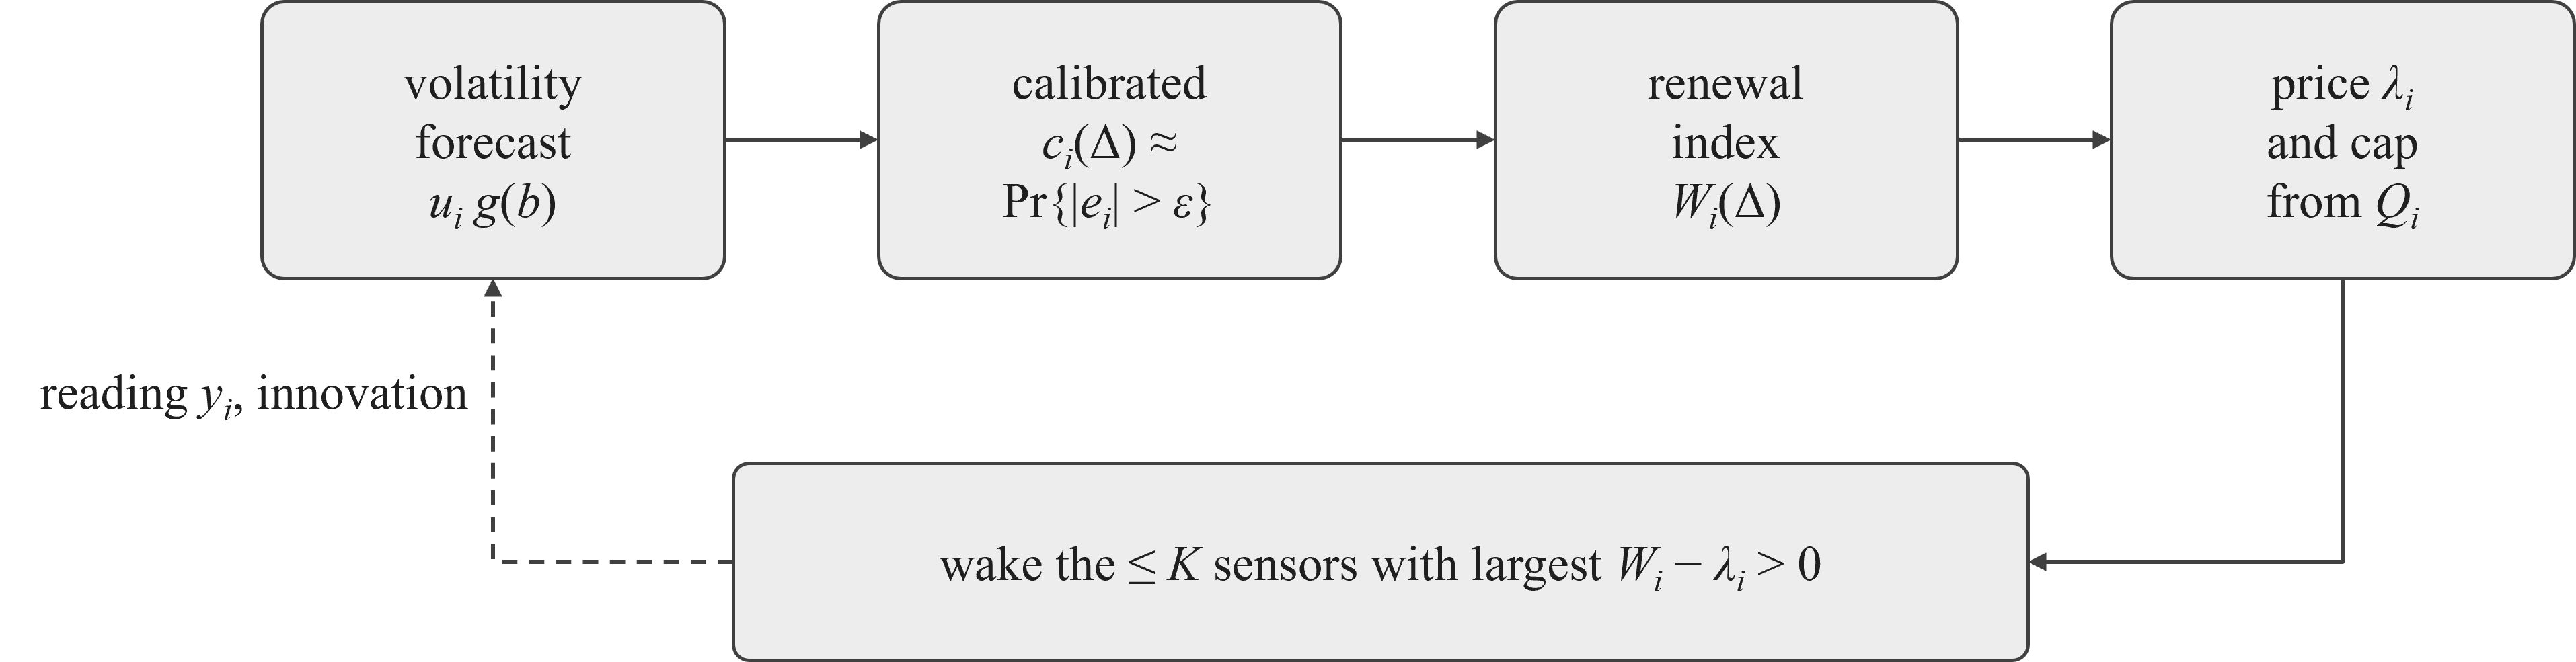
\includegraphics[width=\columnwidth]{fig_pipeline.png}
\caption{FG-Wake at the sink. Readings from polled sensors update the
forecaster and the calibration, and polls update the energy queues.}
\label{fig:pipeline}
\vspace{-3mm}
\end{figure}

FG-Wake runs entirely at the sink (Fig.~\ref{fig:pipeline}). The sensors only
need an addressable WuRx.

\subsection{Volatility forecast from irregular polls}
When sensor $i$ is polled after $\Delta$ slots, the sink observes the innovation
$r=y_i-\hat x_i(t)$. Under a locally diffusive model, $\mathbb{E}[r^2]$ is about
the volatility integrated over the interval, so each poll is a noisy measurement
of it. We factor the per-slot volatility as $u_i\,g(b)$. Here $u_i$ is a
per-sensor scale, and $g(b)$ is a time-of-day profile over $B$ bins, where
$b(t)$ is the bin of slot $t$. The profile is shared by all sensors (to capture
common drivers such as heating, ventilation, and air-conditioning schedules) and
normalised to mean one. The sink keeps
$G_i$, the sum of $g(b(t))$ over the slots since the last poll, and on each poll
updates
\begin{equation}
u_i\leftarrow(1-\omega)\,u_i+\omega\,r^2/G_i,\qquad
\omega=\begin{cases}\omega_{\uparrow} & \text{if } r^2/G_i>u_i\\ \omega_{\downarrow}&\text{otherwise,}\end{cases}
\end{equation}
which reacts fast to bursts ($\omega_\uparrow>\omega_\downarrow$). It also moves
the bins from that of the previous poll to the one following the interval (at
least two bins) towards $(r^2/\Delta)/u_i^-$ with step $\beta$, where $u_i^-$ is
the scale before this update. The predicted error variance is
$v_i=u_iG_i+2\sigma_n^2$.

\subsection{Online calibration of the violation probability}
A Gaussian error would give $\Pr\{|e_i|>\epsilon\}=\mathrm{erfc}(\epsilon/\sqrt{2v_i})$,
where $\mathrm{erfc}$ is the complementary error function. Real processes are often drift-dominated and heavy-tailed, however. On the Intel
trace, this Gaussian prediction averages \CalGaussPred{} at the moments when the
sink polls, while the observed violation frequency at those moments is
\CalGaussObs. FG-Wake therefore learns the probability directly:
\begin{equation}\label{eq:calib}
c_i(\Delta)=\sgm\!\big(\theta_0+\theta_1\ln(v_i(\Delta)/\epsilon^2)+\theta_2\ln(\rho\Delta)\big),
\end{equation}
where $\sgm(z)=1/(1+e^{-z})$. Each poll yields a labelled sample
$(v_i,\Delta,\mathbb{1}\{|r|>\epsilon\})$ at the age at which it was taken. In
every slot with polls, $\theta$ takes one stochastic-gradient step on the
log-loss (rate $\eta$), using the mean gradient over the polled sensors. It is
pooled over sensors and initialised to a logistic fit of the erfc curve over
$\ln(v/\epsilon^2)\in[-6,3]$. We
project $\theta_1\ge0.2$ and $\theta_2\ge0$, so that $c_i$ is non-decreasing in
variance and in age; Section~\ref{sec:results} shows what happens without the
projection. With calibration, the mean prediction at poll times is \CalFgPred{}
against an observed \CalFgObs.

\subsection{The value of polling now}
Ranking sensors by $c_i$ is myopic. A very volatile sensor is likely to violate
the tolerance now, but a poll buys it only a few compliant slots. Consider a
single sensor whose violation probability $c(k)$ at age $k$ is known and
non-decreasing, and a price $\lambda$ per poll. Polling with period $\tau$
gives the long-run cost $J(\tau)=\big(\sum_{k=1}^{\tau}c(k)+\lambda\big)/\tau$ per
slot.
\begin{proposition}\label{prop:index}
Let $W(\tau)=\tau\,c(\tau+1)-\sum_{k=1}^{\tau}c(k)$. Then $W$ is non-decreasing,
and $\tau^\star=\min\{\tau: W(\tau)\ge\lambda\}$ minimises $J$ over all
periods ($\tau^\star=\infty$, i.e., never poll, if the set is empty).
\end{proposition}
\begin{IEEEproof}
$J(\tau+1)\ge J(\tau)\iff \tau\,c(\tau+1)\ge\sum_{k\le\tau}c(k)+\lambda\iff W(\tau)\ge\lambda$,
and $W(\tau+1)-W(\tau)=(\tau+1)\big(c(\tau+2)-c(\tau+1)\big)\ge0$. Hence $J$
decreases while $W<\lambda$ and is non-decreasing afterwards.
\end{IEEEproof}
$W(\tau)$ is the price at which polling at age $\tau$ and polling one slot later
are equally good. FG-Wake evaluates $W_i=\Delta_i\,c_i(\Delta_i+1)-C_i$ for every
sensor, where $C_i=\sum_{k\le\Delta_i}c_i(k)$ is accumulated slot by slot. If a
sensor's violation probability saturates within a few slots, then
$W_i\le\sum_k(1-c_i(k))$ stays small and the sensor is not favoured. We cap
$\rho W_i$ at $\bar w$. With a time-varying profile $g$ the cost curve is not
stationary, so Proposition~\ref{prop:index} motivates the index rather than proving
FG-Wake optimal.

\subsection{Per-sensor energy prices}
Each sensor has a virtual queue $Q_i(t+1)=\max\{Q_i(t)+a_i(t)-\rho,\,-S\}$ with
$Q_i(0)=0$, which tracks how far it is ahead of ($Q_i>0$) or behind ($Q_i<0$) its
budget. The floor lets up to $S$ unused polls be saved, e.g., overnight. A sensor
may be polled only while $Q_i<S$, i.e., it may borrow fewer than $S+1$ polls. Its
price is $\lambda_i=(Q_i+S)/(\rho V)$. In each slot the sink wakes the (at most
$K$) eligible sensors with the largest positive $\rho W_i-(Q_i+S)/V$, which may
be none (Algorithm~\ref{alg:fgw}).
\begin{proposition}\label{prop:budget}
For every sensor and every horizon $T$,
$\sum_{t<T}a_i(t)<\rho T+S+1$, and over any window of $L$ slots the sensor is
polled fewer than $\rho L+2S+1$ times.
\end{proposition}
\begin{IEEEproof}
Polls need $Q_i<S$ and raise $Q_i$ by less than 1, while the update is otherwise
non-increasing. So $-S\le Q_i(t)<S+1$ for all $t$. Summing
$Q_i(t+1)\ge Q_i(t)+a_i(t)-\rho$ over the window gives
$\sum a_i\le\rho L+Q_i(\text{end})-Q_i(\text{start})$.
\end{IEEEproof}
This is the standard virtual-queue argument~\cite{neely2010}, here with a hard
cap. The cap makes the bound independent of $V$, which then only sets how strongly
the price reacts.

\begin{algorithm}[t]
\caption{FG-Wake, executed by the sink in slot $t$}\label{alg:fgw}
\begin{algorithmic}[1]
\For{each sensor $i$} \Comment{$O(N)$}
\State $G_i\!\mathrel{+}=g(b(t))$;\; $v_i\gets u_iG_i+2\sigma_n^2$;\; compute $c_i(\Delta_i)$, $c_i(\Delta_i{+}1)$ by \eqref{eq:calib}
\State $C_i\!\mathrel{+}=c_i(\Delta_i)$;\; $W_i\gets\min\{\Delta_i c_i(\Delta_i{+}1)-C_i,\ \bar w/\rho\}$
\State $s_i\gets\rho W_i-(Q_i+S)/V$ if $Q_i<S$, else $s_i\gets-\infty$
\EndFor
\State $\mathcal{A}\gets$ the $\le K$ sensors with the largest $s_i>0$ \Comment{$O(N)$ selection}
\For{$i\in\mathcal{A}$} wake $i$; receive $y_i$; update $\hat x_i$, $u_i$, $g$ ($O(B)$); reset $G_i,C_i$
\EndFor
\State one gradient step on $\theta$ if $\mathcal{A}\neq\emptyset$; $Q_i\gets\max\{Q_i+\mathbb{1}\{i\in\mathcal{A}\}-\rho,-S\}$ $\forall i$
\end{algorithmic}
\end{algorithm}

%======================================================================
\section{Implementation and Experimental Setup}\label{sec:setup}
%======================================================================
\textbf{Simulator.} We implemented a slot-level simulator of
Section~\ref{sec:model} in Python~\PyVer{} with NumPy~\NpVer. One slot is one
minute, and Table~\ref{tab:params} lists all parameters. The code (all policies,
data preparation, and the scripts that produce every number, table and figure in
this paper) will be released with the camera-ready version.

\begin{table}[t]
\centering
\caption{Simulation parameters (defaults; sweeps in Section~\ref{sec:results}).}
\label{tab:params}
\footnotesize
\setlength{\tabcolsep}{4pt}
\begin{tabular}{@{}l@{\hspace{4pt}}>{\raggedright\arraybackslash}p{0.60\columnwidth}@{}}
\toprule
Slot; horizon & 1 min; trace: 10 days (1 warm-up + 9); synthetic: 11 days (1 + 10)\\
Budget $\rho$; capacity $K$ & 1/30 polls/slot; $\lceil 3N\rho\rceil$\\
Tolerance $\epsilon$; sensing cost $\alpha$ & 0.5 ($^\circ$C on the trace); 1\\
Trace & 28 motes ($K{=}3$); held-out 8 motes ($K{=}1$)\\
Synthetic & $N{=}100$, $\sigma_0{=}0.01$, $\sigma_n{=}0.02$, 20 seeds (sweeps: 3--10)\\
FG-Wake forecaster & $B{=}48$, $\beta{=}0.02$, $\omega_\uparrow{=}0.5$, $\omega_\downarrow{=}0.2$\\
Index, price, learning & $\bar w{=}2$, $S{=}10$, $V{=}200$, $\eta{=}0.01$ (validated)\\
Trend smoothing $\gamma$ & 0.3 (trace, all policies)\\
DPS grid & $T_s\in\{1,2,\dots\}$ up to $1/\rho$, including $\lfloor1/\rho\rfloor,\lceil1/\rho\rceil$; $\kappa\in\{0.2,0.5,0.7,1\}$, $S'\in\{10,40\}$\\
Schedules & rate$_h\propto p_h^{\,q}$, $q\in\{0,0.125,0.25,0.375,0.5,0.75,1,1.5\}$\\
\bottomrule
\end{tabular}
\vspace{-3mm}
\end{table}


\textbf{Intel Lab trace.} The Intel Berkeley Research Lab data~\cite{intellab2004}
come from 54 motes. Of the \IntelRows{} rows in the file, \IntelParsed{} parse to
motes 1--54. Keeping temperatures in $[5,45]^\circ$C with supply voltage
$\ge2.3$\,V leaves \IntelClean{} readings; dying motes report values such as
$122^\circ$C. We average these per mote into 1-minute bins. The \emph{main window}
is the 10-day window with the most motes observed in $\ge80\%$ of minutes
(\IntelStart, \IntelMotes{} motes, \IntelObs\% of mote-minutes observed). The
\emph{held-out window} is the best such window starting on or after 10~March
(\HoStart, \HoMotes{} motes, \HoShared{} of them also in the main set,
\HoObs\% observed). Minutes without a reading are handled conservatively. A poll
(or a push-side sample) in such a minute fails: it costs energy but returns
nothing. These minutes are not scored, so no information from interpolated values
reaches the sink or the metrics. The
trace is superdiffusive: the variance of temperature changes grows with the lag
as $h^{\IntelExpNight}$ at night and $h^{\IntelExpDay}$ by day. All policies on it,
including the push baseline, therefore use the trend estimator
($\gamma=0.3$). Readings are used as recorded ($\sigma_n=0$), and
$\epsilon=0.5^\circ$C.

\textbf{Synthetic data.} Each sensor follows a random walk with per-slot standard
deviation $\sigma_0 z_i m(t)\zeta_i(t)$. Here $z_i$ is log-uniform in $[0.5,2]$;
$m(t)=6$ between 07:00 and 19:00 and 1 otherwise, with a per-sensor shift of
$\pm60$\,min; and $\zeta_i(t)\in\{1,4\}$ is a Markov burst process (start
probability $1/2000$, mean length 60 slots). With $\sigma_0=0.01$, $\epsilon=0.5$,
$\sigma_n=0.02$, $N=100$, 11 days and the zero-order hold, this setting has a
strictly daily volatility pattern and allows a \emph{genie} variant that knows
the true variance.

\textbf{Defaults and protocol.} $\rho=1/30$, $\alpha=1$, and $K=\lceil3N\rho\rceil$,
which is \SyHead, \TrHead{} and \HoHead{} times the aggregate budget on the
synthetic, main and held-out data. The first day is warm-up and is not scored.
The credit/debt window is fixed to $S=\ValS$ polls, about five hours of budget.
$(V,\eta,B)=(\ValV,\ValLr,\ValB)$ were selected by grid search on five synthetic
validation seeds that are disjoint from the test seeds. The design (trend
estimator, calibration layer, shared profile) was, however, developed while
inspecting the main trace window, and preliminary runs explored parameter values
on it. Only the held-out window was untouched by design and tuning. Synthetic
results are means over \SyNseeds{} test seeds with 95\% confidence intervals
(CIs). The trace results come from single deterministic runs, so per-day
statistics are descriptive.

\textbf{Baselines.} All use the same estimator and budget.
\emph{RR}: periodic polling every $1/\rho$ slots with staggered phases. For a fixed
number of polls, it minimises the mean AoI.
\emph{Schedule (warm-up day)}: each sensor follows an hour-of-day schedule with rate
$\propto p_h^{\,q}$. Here $p_h$ is the standard deviation of that sensor's change
over $1/\rho$ slots starting in hour $h$, measured on the warm-up day only. This
baseline is deployable; $q$ is chosen in hindsight.
\emph{Schedule (hindsight)}: the same family, plus profiles $p_h$ equal to RR's
hourly violation ratio, with profile and $q$ fitted on the evaluation data
itself. It is a reference for the best fixed schedule, not an implementable
policy. With $q=0$, both reduce to periodic polling.
\emph{Random polling (RND)}: Bernoulli($\rho$) wake-ups.
\emph{Maximum-variance polling (MaxVar)}: among sensors holding a token (rate $\rho$, depth $S$), wake the
$K$ with the largest predicted variance $v_i$. This is a greedy rule in the
spirit of the Kalman-filter-based baseline of~\cite{jonah2026fair}.
\emph{DPS}: the push-based scheme of~\cite{santini2006}. Each sensor samples
every $T_s$ slots (cost $\alpha$) and transmits (cost 1) if its reading deviates
from the shared prediction by more than $\kappa\epsilon$ and it holds a token.
Tokens accrue at rate $\rho(1+\alpha)-\alpha/T_s$ up to a depth $S'$. $T_s\le1/\rho$,
$\kappa$ and $S'$ are chosen in hindsight; $T_s=1/\rho$ with a small $\kappa$
reproduces RR.
\emph{Oracle}: knows the current true error and uses FG-Wake's queue and cap. It is
a clairvoyant reference, not an implementable policy.

%======================================================================
\section{Results}\label{sec:results}
%======================================================================
\begin{table*}[t]
\centering
\caption{Violation ratio $\bar v$ (\%), MAE, mean AoI and realised energy relative to the budget ($E/B$) at $\rho=1/30$, $\alpha=1$, $K=\lceil3N\rho\rceil$. Trace metrics use observed minutes only. Synthetic: mean $\pm$ 95\% CI over 20 seeds. Hindsight baselines tune their parameters on the evaluation data itself.}
\label{tab:main}
\setlength{\tabcolsep}{5pt}
\small
\begin{tabular}{@{}lcccccccc@{}}
\toprule
 & \multicolumn{4}{c}{Intel main (28 motes)} & Held-out (8) & \multicolumn{3}{c}{Synthetic ($N{=}100$)}\\
\cmidrule(lr){2-5}\cmidrule(lr){6-6}\cmidrule(l){7-9}
Policy & $\bar v$ & MAE [$^\circ$C] & AoI [min] & $E/B$ & $\bar v$ & $\bar v$ & MAE & $E/B$\\
\midrule
RR (periodic) & 11.67 & 0.269 & 17.6 & 1.00 & 9.65 & 4.16$\pm$0.14 & 0.120 & 1.00\\
Schedule (warm-up day) & 10.57 & 0.247 & 20.2 & 1.00 & 8.72 & 2.89$\pm$0.11 & 0.113 & 1.00\\
Schedule (hindsight) & 9.22 & 0.224 & 22.3 & 1.00 & 7.12 & 2.45$\pm$0.10 & 0.111 & 1.00\\
RND & 20.69 & 0.538 & 33.0 & 0.99 & 20.86 & 7.51$\pm$0.17 & 0.160 & 1.00\\
MaxVar & 11.94 & 0.270 & 17.6 & 1.00 & 9.67 & 4.15$\pm$0.13 & 0.120 & 1.00\\
DPS (push, hindsight) & 9.97 & 0.251 & 34.8 & 0.95 & 7.52 & 3.19$\pm$0.12 & 0.144 & 0.92\\
\midrule
\textbf{FG-Wake} & \textbf{9.88} & 0.342 & 23.9 & 1.01 & \textbf{7.73} & \textbf{3.03$\pm$0.11} & 0.113 & 0.99\\
\quad without time-of-day shape & 7.94 & 0.218 & 19.8 & 1.00 & 7.75 & 3.28$\pm$0.11 & 0.113 & 0.99\\
\quad without calibration (Gaussian) & 14.70 & 0.749 & 35.2 & 1.01 & 8.01 & 3.03$\pm$0.11 & 0.117 & 0.99\\
\quad without renewal index (myopic) & 10.85 & 0.268 & 24.7 & 1.01 & 9.01 & 3.61$\pm$0.12 & 0.125 & 0.99\\
\quad without projection & 9.52 & 0.278 & 22.4 & 1.01 & 7.94 & 3.02$\pm$0.10 & 0.113 & 0.99\\
\quad frozen after warm-up & 12.57 & 0.268 & 19.0 & 0.98 & 10.12 & 3.54$\pm$0.10 & 0.118 & 0.99\\
\quad without debt cap & 12.01 & 0.690 & 33.2 & 1.02 & 19.56 & 3.02$\pm$0.11 & 0.113 & 0.99\\
\quad genie variance & -- & -- & -- & -- & -- & 2.71$\pm$0.10 & 0.120 & 0.99\\
\midrule
Oracle (clairvoyant) & 2.22 & 0.189 & 35.2 & 1.01 & 2.38 & 0.15$\pm$0.02 & 0.098 & 1.00\\
\bottomrule
\end{tabular}
\vspace{-3mm}
\end{table*}


\textbf{Main comparison.} Table~\ref{tab:main} gives the default operating point.
On the main trace window, FG-Wake lowers the violation ratio from \TrRR\% (RR) to
\TrFG\%, a reduction of \TrRed\%, while spending \TrRateMean{} of the budget. It is
better than RR on \TrDays{} of \TrNdays{} days (per-day difference \TrDiff{}
points; the descriptive 95\% CI \TrDiffCI{} includes zero). On the held-out
window the reduction is
\HoRed\% (better on \HoDays{} of \HoNdays{} days). On synthetic data it is
\SyRed\% (paired per-seed 95\% CI \SyRedCI\%). On the main window, \TrFailRR\% of
RR's polls and \TrFailFG\% of FG-Wake's hit a minute without a reading
(\HoFailRR\% and \HoFailFG\% on the held-out window), because FG-Wake retries
sensors whose readings are missing. FG-Wake targets time out of tolerance, not
average error or freshness, and it trades one for the other. On the trace its MAE
is \TrMaePct\% \emph{higher} than RR's (\TrMaeFG{} versus \TrMaeRR\,$^\circ$C), and its
mean AoI is \TrAoiPct\% higher: when it leaves a quiet sensor unpolled, the
errors that do occur grow larger.
Across all FG-Wake runs, the largest per-sensor overshoot within an evaluation
window is \OverMax{} polls, below the bound $2S{+}1=\BoundWin$ of
Proposition~\ref{prop:budget}.

\textbf{Schedules and push.} With spare capacity, MaxVar polls each sensor as
soon as a token is available and behaves like RR (\TrMV\% on the trace), so greedy
ranking alone does not shift budget in time. A schedule calibrated on the warm-up
day reduces violations by \TrSchedCRed\% and \HoSchedCRed\% on the two trace
windows, less than FG-Wake. A schedule fitted in hindsight (best profile:
\TrSchedBStat, $q=\TrSchedBExpo$) reduces them by \TrSchedBRed\% and
\HoSchedBRed\%, \emph{more} than FG-Wake. On the synthetic data, with its strictly
daily pattern, even the warm-up-day schedule (\SySchedCRed\%) beats FG-Wake
(\SyRed\%), and the hindsight schedule reaches \SySchedBRed\%. The
hindsight-tuned push scheme (DPS, $\alpha=1$) reduces violations by \TrDpsRed\%
and \HoDpsRed\% on the trace windows, on par with FG-Wake, and by \SyDpsRed\% on
synthetic data. In short, FG-Wake learns online much, but not all, of what a
schedule fitted with hindsight knows.

\begin{figure}[t]
\centering
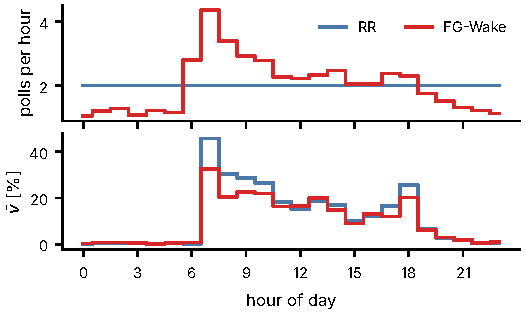
\includegraphics[width=\columnwidth]{fig_hourly.pdf}
\vspace{-6mm}
\caption{Where the budget goes on the Intel trace ($\rho=1/30$): polls per sensor
and hour (top) and violation ratio (bottom) by hour of day, over the nine
evaluation days.}
\label{fig:hourly}
\vspace{-3mm}
\end{figure}

\textbf{Where the polls go.} FG-Wake moves polls from the quiet night to the day
(Fig.~\ref{fig:hourly}). The share of polls between 20:00 and 07:00 drops from
\NightRR\% (RR) to \NightFG\%. FG-Wake peaks at \PeakFG{} polls per hour at
\PeakHourFG, and in that hour its violation ratio is \PeakVFG\% against
\PeakVRR\% for RR. Hours 07:00--10:59 account for \GainMorning\% of the net
reduction in violations (\GainMorningGross\% of the gross). FG-Wake is worse than
RR in \HoursWorse{} of the 24 hours, \HoursWorseNight{} of them at night. Most of
the violation-minutes it loses (\LossTopShare\%), however, fall at
\LossTopHours; at \LossWorstHour, for example, it reaches \LossWorstFG\% against
\LossWorstRR\%.

\textbf{What matters.} The ablation rows of Table~\ref{tab:main} remove one
component at a time.
\begin{itemize}
\item \emph{Calibration.} Without it (\emph{Gaussian}), FG-Wake is worse than RR
on the main window (\TrGauss\%), slightly worse than FG-Wake on the held-out window
(\HoGauss\%), and equal on synthetic data (\SyGauss\%). On the main window, the
expected calibration error of the violation probability at poll times is
\EceGauss{} for the Gaussian model and \EceFg{} with calibration.
\item \emph{Renewal index.} Ranking by the myopic $c_i$ (with its own validated
$V,\eta$) shrinks the reduction to \TrMyoRed\%, \HoMyoRed\% and \SyMyoRed\%.
\item \emph{Projection and shape.} Both have mixed effects. Without the
projection: \TrNoProj\% (main), \HoNoProj\% (held-out), \SyNoProj\% (synthetic).
Without the shared time-of-day shape: \TrShape\%, \HoShape\% and \SyShape\%.
Validation selected the shape, which costs accuracy on the main window.
\item \emph{Online learning.} Freezing the learner after the warm-up day makes
FG-Wake worse than RR on both trace windows (\TrStatic\%, \HoStatic\%).
\item \emph{Debt cap.} Without it, FG-Wake keeps retrying sensors during long
data gaps. \TrNoCapFail\% and \HoNoCapFail\% of its polls fail, and the violation
ratio rises to \TrNoCap\% and \HoNoCap\%. On synthetic data, where no reading is
missing, the cap changes nothing (\SyNoCap\%). Besides guaranteeing the budget,
the cap limits the energy wasted on unreachable sensors.
\item \emph{Variance knowledge.} On synthetic data, the genie that knows the true
variance reduces violations by \SyGenieRed\%, against \SyRed\% for FG-Wake.
\item \emph{Parameters.} Across the five best validated $(V,\eta,B)$, the reduction
ranges from \RobTrMin\% to \RobTrMax\% on the main window and from \RobHoMin\% to
\RobHoMax\% on the held-out window.
\end{itemize}

\begin{figure}[t]
\centering
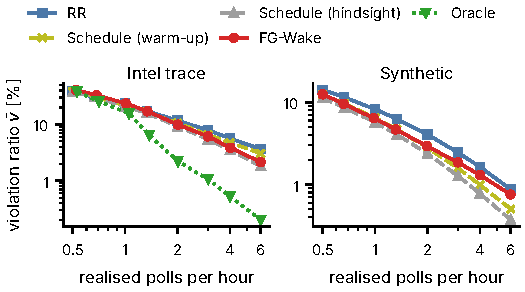
\includegraphics[width=\columnwidth]{fig_budget.pdf}
\vspace{-6mm}
\caption{Violation ratio versus the \emph{realised} poll rate as the budget $\rho$
sweeps from one poll per 10\,min to one per 2\,h ($K=\lceil3N\rho\rceil$). Left:
Intel trace. Right: synthetic data (10 seeds; 95\% CI half-widths at most
\BudSyCiMax\% of the mean; the oracle is omitted for clarity).}
\label{fig:budget}
\vspace{-3mm}
\end{figure}

\textbf{Budget.} Fig.~\ref{fig:budget} plots accuracy against the energy actually
spent. To reach RR's accuracy at $\rho=1/30$, FG-Wake needs \TrSave\% fewer
wake-ups on the trace and \SySave\% fewer on synthetic data (log--log
interpolation; \TrSaveLin\% and \SySaveLin\% with linear interpolation). If
per-reading energy dominates, \TrSave\% fewer wake-ups extend the battery lifetime
by \TrLife\%. On the trace, FG-Wake beats RR down to \BudTrWinMin{} polls per hour
and loses below that: \BudTrFgLow\% versus \BudTrRrLow\% at 0.5 polls per hour, where it
also overspends by \BudTrFgRateLowMax$\times$ on average (worst sensor
\BudTrFgSensorLowMax$\times$). With a zero-order hold for both, RR still wins at
that budget (\LbRRzoh\% versus \LbFGzoh\%). On the trace, the hindsight schedule
beats FG-Wake at \BudTrSchedBBeatsFg{} of the \BudN{} budgets. The warm-up-day
schedule beats it at the \BudTrSchedCBeatsFg{} lowest budgets and loses at the
others.

\begin{figure}[t]
\centering
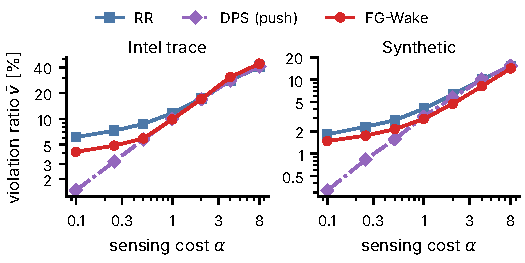
\includegraphics[width=\columnwidth]{fig_alpha.pdf}
\vspace{-6mm}
\caption{Pull versus push at equal energy per sensor (budget $2/30$ units per
slot) as the sensing cost $\alpha$ grows relative to a transmission. DPS uses the
best $T_s$, $\kappa$ and token depth in hindsight; pull policies use
$\rho=\frac{2}{30}/(1+\alpha)$, and RR's integer period gives 0.99--1.03 of the
budget. Synthetic: mean of 3 seeds; trace: single run.}
\label{fig:alpha}
\vspace{-3mm}
\end{figure}

\textbf{When to pull and when to push.} Fig.~\ref{fig:alpha} fixes the energy
budget and varies $\alpha$. DPS must sense in order to decide whether to transmit.
When sensing is cheap it samples often and wins clearly: at $\alpha=\AlphaMin$,
it reaches \TrDpsLowAlpha\% against \TrFgLowAlpha\% for FG-Wake on the trace, and
\SyDpsLowAlpha\% against \SyFgLowAlpha\% on synthetic data. As $\alpha$ grows, its
sensing budget shrinks, while FG-Wake decides when to sense without sensing. On
synthetic data FG-Wake is better for $\alpha\gtrsim\AlphaLoSy$. On the trace,
DPS matches or beats FG-Wake at every $\alpha$ tested, except at $\alpha=1$, where
they are within a tenth of a point (\TrFG\% versus \TrDPS\%). At $\alpha=\AlphaMax$
(\BudHighAlpha{} polls per hour), FG-Wake reaches \TrFgHighAlpha\% against
\TrDpsHighAlpha\% for DPS and \TrRrHighAlpha\% for RR. Pulling therefore pays off
only for costly sensing at budgets adequate for the tolerance. Push also needs no
WuRx, whose listening cost is not modelled.

\textbf{Capacity, tolerance and run time.} On the trace (single runs), $K=1$
(\HeadCapTrOne$\times$ the aggregate budget) gives $\HeadTrOne$\%, $K=2$ gives
\HeadTrOneHalf\%, $K=3$ gives \HeadTrThree\% and $K=5$ gives \HeadTrFive\%, so the
gain needs some spare capacity. On synthetic data it stays between \HeadSyMin\% and
\HeadSyMax\%. The tolerance matters more. Relative to RR, FG-Wake changes the
violation ratio by $\EpsTrQ$\%, \EpsTrH\% and \EpsTrOne\% on the main window for
$\epsilon=0.25$, 0.5 and $1\,^\circ$C, and by $\EpsHoQ$\%, \EpsHoH\% and
\EpsHoOne\% on the held-out window (positive values are reductions). On the
trace, FG-Wake loses in every configuration we tested in which RR is out of
tolerance more than \RegimeThr\% of the time, and also at $\epsilon=0.25\,^\circ$C
and $K=1$. Where RR is between about 17\% and \RegimeThr\%, FG-Wake's wins are
below a quarter point. Algorithm~\ref{alg:fgw},
including the learning updates, takes \RtFGsmall, \RtFGmid{} and
\RtFGbig\,$\mu$s per slot for $N=28$, 100 and 1000 in our unoptimised NumPy code on
one core of a cloud virtual machine. This is negligible for one-minute slots.

%======================================================================
\section{Discussion and Limitations}\label{sec:disc}
%======================================================================
Our results bound what online wake-up polling buys. On real data, FG-Wake's gain
over periodic polling is a time-of-day reallocation of the budget that it learns
online. It beats a schedule calibrated on one day of data, but a schedule fitted
in hindsight does better. On data with a strictly daily pattern, even the
one-day schedule wins. A push scheme tuned in hindsight is on par at moderate
sensing cost and clearly better when sensing is cheap. FG-Wake is thus most
useful when no prior profile is available, sensing is costly, and the budget is
adequate for the tolerance. When periodic polling is out of tolerance about
20\% of the time or more, FG-Wake gains nothing and should fall back to it.
Combining a schedule prior with FG-Wake's online correction is a natural next
step.

The study has further limitations. The results come from trace-driven
simulation, not from a WuRx testbed. Medium access control losses, wake-up
latency and the WuRx listening power (about $0.1\,\mu$W to tens of
microwatts~\cite{piyare2017,magno2016})
are not modelled; the last matters for the push comparison and for the absolute
lifetime gain. The trace covers one building, one quantity and a held-out window
of only \HoMotes{} motes, and the design was developed on the main window. The
results are sensitive to parameters and design details (see \emph{What matters}).
For example, updating the shared profile with the scale \emph{after} rather than
before its update gives \SvTrPost\% instead of \SvTrPre\% on the main window.
Proposition~\ref{prop:index} covers a single sensor with a known, stationary cost
curve; with learned curves, a time-varying profile and the coupling through $K$,
FG-Wake is a heuristic. Finally, we compare against a variance-greedy proxy rather
than a re-implementation of the online AoII Whittle policy
of~\cite{jonah2026fair}. A head-to-head comparison is an important next step.

%======================================================================
\section{Conclusion}
%======================================================================
FG-Wake shows that a sink with a wake-up radio can learn online where to spend
per-sensor wake-up budgets, with a hard budget guarantee and little computation.
It combines a calibrated forecast of when each sensor's estimate will leave its
tolerance, an index that weighs polling now against waiting, and per-sensor
energy prices. On real indoor-temperature data at two polls per hour, it reduced
tolerance violations by \TrRed\% (\HoRed\% on a held-out window) at equal energy,
and it beat a schedule calibrated on a warm-up day. A schedule fitted in hindsight
did better, push sensing is preferable when sensing is cheap, and FG-Wake does
not help when the budget is too small for the tolerance. Future work includes
schedule priors, a WuRx testbed, a head-to-head comparison with online
Whittle-index polling, and joint pull/push operation.

\section*{Acknowledgment}
This research was conducted as part of the AI4GovAccelerate (AI4GOV-X) project
No.~101190043, under Research Contract No.~29EUD 2026. The authors acknowledge the
institutional and research support provided within the framework of this project.

\bibliographystyle{IEEEtran}
\bibliography{refs}

\end{document}
